\documentclass[12pt,a4paper]{report}
\usepackage{mathptmx}

\usepackage[slovak]{babel}
\usepackage[utf8]{inputenc}
\usepackage{setspace}

\usepackage{graphicx}
\onehalfspacing

\usepackage{booktabs}
 
\usepackage{enumerate}
\parindent=0pt

\renewcommand{\arraystretch}{1.5}


% chapters bez nadpisov "chapter #"
\usepackage{titlesec}

\setlength\aftertitleunit{\baselineskip}

\titleformat{\chapter}[display]
  {\normalfont\huge\bfseries}{}{0pt}{\Huge}
\titleformat{name=\chapter,numberless}[display]
  {\normalfont\huge\bfseries}{}{0pt}{\Huge}
\titlespacing*{\chapter}{0pt}{50pt}{*2}
\usepackage[top=2.5cm, bottom=2.5cm, right=2cm, left=3.5cm]{geometry}  %okraje
\usepackage{listings}


\lstdefinestyle{mystyle}{
    backgroundcolor=\color{backcolour},   
    commentstyle=\color{codegreen},
    keywordstyle=\color{magenta},
    numberstyle=\tiny\color{codegray},
    stringstyle=\color{codepurple},
    basicstyle=\footnotesize,
    breakatwhitespace=false,         
    breaklines=true,                 
    captionpos=b,                    
    keepspaces=true,                 
    numbers=left,                    
    numbersep=5pt,                  
    showspaces=false,                
    showstringspaces=false,
    showtabs=false,                  
    tabsize=2
}
 
\lstset{style=mystyle}
 
\begin{document}
\pagestyle{empty}


\def\skola{Univerzita Komenského v Bratislave} 
\def\fakulta{Fakulta matematiky, fyziky a informatiky} 
\def\nazov{Decentralizovaná a distribuovaná komunikačná platforma} 
\def\autor{Adam Horváth}

%\pagestyle{empty} 

\begin{center} 
\scshape\Large 
\skola\\ 
\fakulta\\ 
\vspace*{\fill} 
\bfseries\Large 
\nazov \\[10pt] \mdseries\large 
bakalárska práca\\ 
\end{center} 

\vspace*{\fill} 
\begin{flushleft} 
\large Autor: \autor \\ 
Školiteľ: RNDr. Jozef Šiška \\ 
Bratislava, 2014\\ 
\end{flushleft}



\tableofcontents
\thispagestyle{empty}
\addtocontents{toc}{\protect\thispagestyle{empty}}



\setcounter{page}{0}
\pagestyle{plain}

\chapter{Úvod}
Napriek tomu, že v súčasnosti existujú multiagentové systémy viac-menej v pozadí verejného záujmu, v praktickom využití nachádzajú svoje miesto. Spomenúť môžeme napríklad tému na vzostupe - „inteligentné domy“, kde navzájom prepojené agenty starajúci sa o rôzne súčasti domu sú schopní konať na základe stavu podmienok vo svojom prostredí. 
Ďalším objektom záujmu tejto práce bude decentralizovanosť týchto systémov. Od platformy LCP sa očakáva, že bude multiagentová a taktiež má existovať bez centrálnej autority, v tomto prípade servera. Pre našu komunikačnú platformu, to znamená, že má byť schopná nakonfigurovať sa sama od seba.
\newline

\section{Motivacia}
\section{Cieľ práce}
Cieľom tejto práce je rozšírenie Jednoduchej Komunikačnej Platformy (ďalej LCP, podľa „Lightweight Communication Platform“) o možnosť komunikácie agentov v jednej lokálnej sieti s agentami v inej lokálnej sieti. Východiskovým riešením tohto problému je takzvaný „Gateway Agent“, ktorý je schopný posielať správy aj za iných agentov v jeho lokálnej sieti a prakticky sa správa ako virtuálny router.
\newline
\section{Štruktúra práce}
Táto práca bude ďalej rozčlenená do siedmich častí. Prvá kapitola začne základnou definíciou pojmu agent a jeho členenie. Za definíciou budú nasledovať teoretické (kapitola 1) a technické (kapitola 2) základy a komunikácia agentov v multiagentových systémoch. V ďalšej časti sa budeme venovať podobným, už existujúcim riešeniam problematiky a príkladom multiagentových alebo decentralizovaných systémov (kapitola 3). Následne popíšeme technológie, ktoré budú použité v riešení ako aj technológie, ktoré budú slúžiť ako inšpirácia pri vytváraní riešení možných problémov (kapitola 4). Tým sa dostaneme k jadru tejto práce a to podrobný popis cieľa, ktorý má byť výsledkom tejto práce (kapitola 5). Táto kapitola bude nasledovaná popisom riešenia hlavného problému a implementáciou tohto riešenia (kapitola 6). V závere v krátkosti zhrnieme výsledok, ku ktorému sme sa dopracovali v tejto práci (kapitola 7).  
\newline

\chapter{Prehľad}
	Kvôli tomu, aby sme dokázali plne pochopiť, čo sa budeme snažiť v tejto práci dosiahnuť a pre celkové porozumenie problematiky sa budeme v tejto časti práce venovať prehľadu poznatkov z oblasti agentov a multiagentových systémov. Práve preto musíme najskôr definovať pojem agent a vysvetliť teoretické základy multiagentových systémov a ich potenciál, ktorý sa budeme snažiť načrtnúť na príkladoch ich praktického využitia vo svete. 
\newline
\section{Inteligentný agent}
	Klasickú definíciu agenta nám ponúkajú Russel a Norvig:
„Agent je všetko, na čo sa dá pozerať ako na niečo, čo vníma svoje okolie senzormi a reaguje na toto okolie pomocou aktuátorov.“ 
Agent je podľa nich zložený z architektúry a agentového programu, ktorého vytvorenie je úlohou práve umelej inteligencie. Fyzická architektúra nás v tejto práci nebude zaujímať, preto ďalej v tejto kapitole budeme rozumieť pod pojmom agent práve agentový program. Existujú agenty, ktoré sú veľmi jednoduché, ale aj také, ktoré sú zložité. Podľa ich vnemovej inteligencie a schopnosti ich opäť Russel a Norvig rozdelili do týchto piatich kategórií, ktoré vzápätí rozoberieme podrobnejšie:
\begin{itemize}
	\item
	Jednoduchý reflexný agent
	\item
	Modelovo-založený reflexný agent
	\item
	Cieľovo-založený agent
	\item
	Úžitkovo-založený agent
	\item
	Učenlivý agent
\end{itemize}
\subsection{Simple reflex agent} 
	Tento druh agenta je úplne najjednoduchší. Reaguje totiž len na aktuálny stav jeho prostredia a pritom si neuchováva žiadnu históriu stavov daného prostredia. Tento agent je plne úspešný iba v úplne pozorovateľnom prostredí. Keď sa jedná o čiastočne pozorovateľné prostredie, vo väčšine je tento agent v nekonečnom cykle a jeho správanie je väčšinou podmienené. Ak je splnená podmienka, tak na ňu programovo reaguje (viď Obr. ~\ref{fig:lifecycle}). 

\begin{figure}[h!]
\centering
  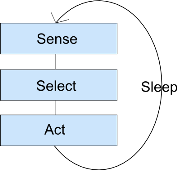
\includegraphics{lifecycle}
  \caption{Diagram cyklu jednoduchého reflexného agenta v čiastočne pozorovateľnom prostredí}
  \label{fig:lifecycle}
\end{figure}


\end{document}






